\documentclass[11pt,largemargins]{homework}

\newcommand{\hwname}{Dwijen Chawra}
\newcommand{\hwemail}{dchawra}
\newcommand{\hwtype}{Homework}
\newcommand{\hwnum}{2}
\newcommand{\hwclass}{CS 251}
\newcommand{\hwlecture}{}
\newcommand{\hwsection}{}

\makeatletter
\renewcommand*\env@matrix[1][\arraystretch]{%
  \edef\arraystretch{#1}%
  \hskip -\arraycolsep
  \let\@ifnextchar\new@ifnextchar
  \array{*\c@MaxMatrixCols c}}
\makeatother

\begin{document}
\maketitle

% question 0 - resources and collaborators statement
\newpage
\setcounter{questionCounter}{-1}
\question
\textbf{Problem 1:} 

Resources used: None

Collaborators: None

\textbf{Problem 2:} 

Resources used: None

Collaborators: None

\textbf{Problem 3:} 

Resources used: None

Collaborators: None

\textbf{Problem 4:} 

Resources used: None

Collaborators: None

\textbf{Problem 5:} 

Resources used: None

Collaborators: None

% Question 1
\newpage
\question
\begin{alphaparts}
    \questionpart
    Represent the expression $((x + 2) ^ 3) * (y - (3 + x)) - 5$ using a binary tree

    % use tikz to draw the tree

    \synttree [- [* [exp [+ [x] [2]] [3]] [- [y] [+ [3] [x]]]] [5]]

    

    \questionpart
    $((x + 2) ^ 3) * (y - (3 + x)) - 5$

    Write this expression in prefix notation using a stack.
    First, we need to convert the expression to prefix notation.
    \begin{verbatim}
- * ^ + x 2 3 - y + 3 x 5
    \end{verbatim}
    Then we reverse it:
    \begin{verbatim}
5 x 3 + y - 3 2 x + ^ * -
    \end{verbatim}
    Then we begin using the stack:

    \newcommand{\customstack}[1]{
        \begin{drawstack}
            % Iterate through the list elements and add them to the stack
            \foreach \element in {#1} {
                \cell{\element}
            }
        \end{drawstack}
    }


\verb|5 x 3 + y - 3 2 x + ^ * -     Stack: []|

\begin{drawstack}
    \cell{}
\end{drawstack}

\verb|x 3 + y - 3 2 x + ^ * -       Stack: [5]|

\customstack{5}

\verb|3 + y - 3 2 x + ^ * -         Stack: [5, x]|

\customstack{5, x}

\verb|+ y - 3 2 x + ^ * -           Stack: [5, x, 3]|

\customstack{5, x, 3}

\verb|Next operator is +, so we pop 3 and x, and push the result of 3 + x|

\verb|y - 3 2 x + ^ * -             Stack: [5, 3 + x]|

\customstack{5, 3 + x}

\verb|- 3 2 x + ^ * -               Stack: [5, 3 + x, y]|

\customstack{5, 3 + x, y}

\verb|Pop the last two elements, and push the result of y - (3 + x)|

\verb|3 2 x + ^ * -                 Stack: [5, y - (3 + x)]|

\customstack{5, y - (3 + x)}

\verb|2 x + ^ * -                   Stack: [5, y - (3 + x), 3]|

\customstack{5, y - (3 + x), 3}

\verb|x + ^ * -                     Stack: [5, y - (3 + x), 3, 2]|

\customstack{5, y - (3 + x), 3, 2}

\verb|+ ^ * -                       Stack: [5, y - (3 + x), 3, 2, x]|

\customstack{5, y - (3 + x), 3, 2, x}

\verb|Pop 2, x, and push the result of 2 + x|

\verb|^ * -                         Stack: [5, y - (3 + x), 3, x + 2]|

\customstack{5, y - (3 + x), 3, x + 2}

\verb|Pop last two, push (x + 2) ^ 3|

\verb|* -                           Stack: [5, y - (3 + x), (x + 2) ^ 3]|

\customstack{5, y - (3 + x), (x + 2) \^{} 3}

\verb|Multiply the last two elements|

\verb|-                             Stack: [5, ((x + 2) ^{} 3) * (y - (3 + x))]|

\customstack{5, ((x + 2)  3) * (y - (3 + x))}

\verb|Pop the last two elements, push the result of the subtraction|

\verb|                              Stack: [((x + 2) ^ 3) * (y - (3 + x)) - 5]|

\customstack{((x + 2) \^{} 3) * (y - (3 + x)) - 5}

    Final result: $((x + 2) ^ 3) * (y - (3 + x)) - 5$


\end{alphaparts}


% Question 2 --------------------------------------------------------------
\newpage
\question

Implementing a dequeue using three stacks. One stack will be for storing the front object, and the other stack will be used to store the back elements. The third stack is a temporary stack used to store values when either front or back stacks are empty.

Assuming that the Stack object has \verb|s.isEmpty()|, \verb|s.push(x)|, \verb|s.pop()| implemented.

\nextverbatimspread{1}
\begin{verbatim}

Dequeue {
    Stack front
    Stack back
    Stack temp

    //allows us to split the stack into two parts when one is empty
    int frontSize
    int backSize
        
    // if both front and back are empty, then the dequeue is empty
    d.isEmpty() {
        return front.isEmpty() && back.isEmpty()
    }

    // just push to the front stack
    d.addFront(x) {
        front.push(x)
        frontSize++
    }

    For remove front, if its not empty, I just pop the value on the top.
    If its empty, in order to reduce the number of times I need to swap, 
        I split the back stack in half and move half to front.
    I use temp as space to store the top of the stack (new back)
    Move the rest of back to front.
    Then move temp back to back.
    Then I pop the value on the top of front.

    d.removeFront() {
        if (frontSize == 0) {
            // this is where we need to split the back stack and move half to front
            newBackSize = int(backSize / 2)

            for i in range(newBackSize):
                temp.push(back.pop()) 
                //this shifted half of back
                //to temp (will become back later)
            
            newFrontSize = backSize - newBackSize

            for i in range(newFrontSize):
                front.push(back.pop()) //shifting the next half to front

            //now we move temp into back

            for i in range(newBackSize):
                back.push(temp.pop())

            frontSize = newFrontSize
            backSize = newBackSize
        }
    }
    
    // just push to the back stack
    d.addBack(x) {
        back.push(x)
        backSize++
    }

    Same logic as removeFront, but we do it for the back stack

    d.removeBack() {
        if (backSize == 0) {
            // this is where we need to split the front stack and move half to back
            newFrontSize = int(frontSize / 2)

            for i in range(newFrontSize):
                temp.push(front.pop()) 
                //this shifted half of front
                //to temp (will become front later)
            
            newBackSize = frontSize - newFrontSize

            for i in range(newBackSize):
                back.push(front.pop()) //shifting the next half to back

            //now we move temp into front

            for i in range(newFrontSize):
                front.push(temp.pop())

            frontSize = newFrontSize
            backSize = newBackSize
        }
    }
}

\end{verbatim}


% Question 3
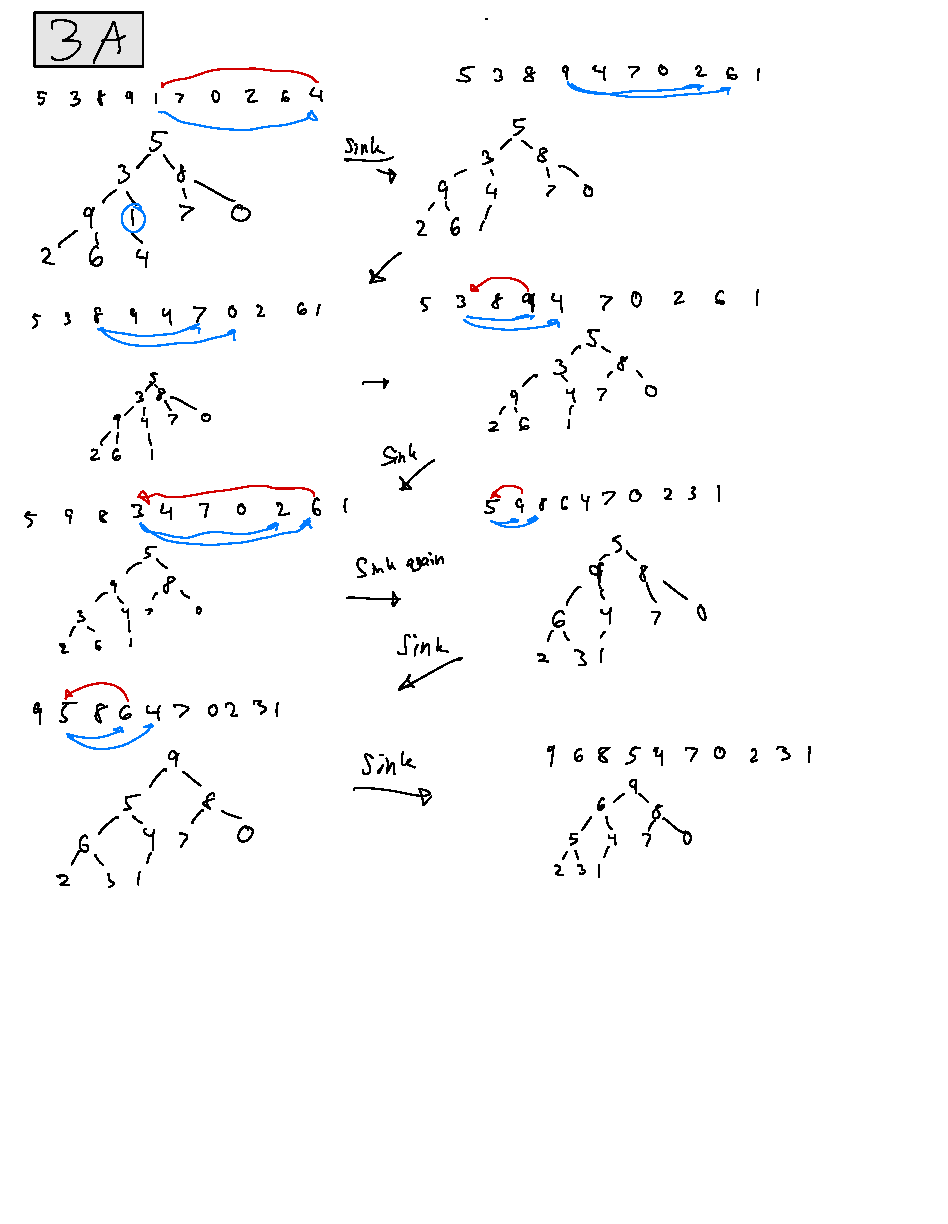
\includepdf[pages=-]{hw2q3.pdf}


% Question 4
\newpage
\setcounter{questionCounter}{3}
\question


Runtime analysis:
Radix sort works on each digit of the number. For each digit, it uses counting sort to sort the numbers. Counting sort has a runtime of O(n + k), where k is the range of the numbers. Since the range of the numbers is 0 to 9, k is a constant. Therefore, the runtime of counting sort is O(n). Since radix sort uses counting sort for each digit, the runtime of radix sort is O(d * n), where d is the number of digits, but d is also constant, so the runtime of radix sort is O(n).

\begin{verbatim}
algorithm CountingSort(A, k)
    let C be an array of length k + 1

    fill C with 0s
    
    let n be the length of array A
    for (i = 0, i < n, 1)
        C[A[i]] = C[A[i]] + 1
    end for
    
    for (i = 1, i <= k, 1)
        C[i] = C[i] + C[i - 1]
    end for
    
    let B be an array of size n
    
    for (i = n - 1, i >= 0, -1)
        B[C[A[i]] - 1] = A[i]
        C[A[i]] = C[A[i]] - 1
    end for
    
    return B
end algorithm


algorithm RadixSort(A)

    let d be the dimension of
    the tuples in A

    for i from d to 1
        CountingSort(A, d) using the
        ith dimension as the key
    end for

end algorithm
\end{verbatim}



% Question 5
\newpage
\question

My approach for this was flawed at first until I found quickselect. First, I calculate the total number of elements in the list. (O(n)) Then, I find the index where the median should be (Kth smallest element), which is the middle index of the list. (O(1)) Then, I use quickselect to find the Kth smallest element. (O(n)).

The total runtime is O(n) + O(1) + O(n) = O(2n) = O(n)

\begin{verbatim}
def median(list):
    n = len(list)
    k = int(n / 2)
    return partition(list, 0, n - 1, k)

def partition(list, l, r, k):

    if l < r:
        pivotIndex = partition(list, l, r)

        if k == pivotIndex:
            return list[k]
        elif k < pivotIndex:
            return partition(list, l, pivotIndex - 1, k)
        else:
            return partition(list, pivotIndex + 1, r, k)
    else:
        return list[l]
\end{verbatim}

\begin{verbatim}
    Dry Run on [38, 12, 31, 1, 34, 15, 11, 48, 24, 23, 3, 47, 4, 32, 35]

    n = 15
    k = 7

    l:  0  r:  14  k:  7
    Partitioning:
    [38, 12, 31, 1, 34, 15, 11, 48, 24, 23, 3, 47, 4, 32, 35]
    [12, 38, 31, 1, 34, 15, 11, 48, 24, 23, 3, 47, 4, 32, 35]
    [12, 31, 38, 1, 34, 15, 11, 48, 24, 23, 3, 47, 4, 32, 35]
    [12, 31, 1, 38, 34, 15, 11, 48, 24, 23, 3, 47, 4, 32, 35]
    [12, 31, 1, 34, 38, 15, 11, 48, 24, 23, 3, 47, 4, 32, 35]
    [12, 31, 1, 34, 15, 38, 11, 48, 24, 23, 3, 47, 4, 32, 35]
    [12, 31, 1, 34, 15, 11, 38, 48, 24, 23, 3, 47, 4, 32, 35]
    [12, 31, 1, 34, 15, 11, 24, 48, 38, 23, 3, 47, 4, 32, 35]
    [12, 31, 1, 34, 15, 11, 24, 23, 38, 48, 3, 47, 4, 32, 35]
    [12, 31, 1, 34, 15, 11, 24, 23, 3, 48, 38, 47, 4, 32, 35]
    [12, 31, 1, 34, 15, 11, 24, 23, 3, 4, 38, 47, 48, 32, 35]
    [12, 31, 1, 34, 15, 11, 24, 23, 3, 4, 32, 47, 48, 38, 35]
    Position of pivot:  11
    Pivot is to the right of k, so we recurse on the left side
    l:  0  r:  10  k:  7
    Partitioning:
    [12, 31, 1, 34, 15, 11, 24, 23, 3, 4, 32, 35, 48, 38, 47]
    [12, 31, 1, 34, 15, 11, 24, 23, 3, 4, 32, 35, 48, 38, 47]
    [12, 31, 1, 34, 15, 11, 24, 23, 3, 4, 32, 35, 48, 38, 47]
    [12, 31, 1, 34, 15, 11, 24, 23, 3, 4, 32, 35, 48, 38, 47]
    [12, 31, 1, 15, 34, 11, 24, 23, 3, 4, 32, 35, 48, 38, 47]
    [12, 31, 1, 15, 11, 34, 24, 23, 3, 4, 32, 35, 48, 38, 47]
    [12, 31, 1, 15, 11, 24, 34, 23, 3, 4, 32, 35, 48, 38, 47]
    [12, 31, 1, 15, 11, 24, 23, 34, 3, 4, 32, 35, 48, 38, 47]
    [12, 31, 1, 15, 11, 24, 23, 3, 34, 4, 32, 35, 48, 38, 47]
    [12, 31, 1, 15, 11, 24, 23, 3, 4, 34, 32, 35, 48, 38, 47]
    Position of pivot:  9
    Right of k, so we recurse on the left side
    l:  0  r:  8  k:  7
    Partitioning:
    [12, 31, 1, 15, 11, 24, 23, 3, 4, 32, 34, 35, 48, 38, 47]
    [1, 31, 12, 15, 11, 24, 23, 3, 4, 32, 34, 35, 48, 38, 47]
    [1, 3, 12, 15, 11, 24, 23, 31, 4, 32, 34, 35, 48, 38, 47]
    Position of pivot:  2
    Left of K, recurse on right side
    l:  3  r:  8  k:  4
    Partitioning:
    [1, 3, 4, 15, 11, 24, 23, 31, 12, 32, 34, 35, 48, 38, 47]
    [1, 3, 4, 11, 15, 24, 23, 31, 12, 32, 34, 35, 48, 38, 47]
    Position of pivot:  4
    Left of K, recurse on right side
    l:  5  r:  8  k:  2
    Partitioning:
    [1, 3, 4, 11, 12, 24, 23, 31, 15, 32, 34, 35, 48, 38, 47]
    Position of pivot:  5
    Left of K, recurse on right side
    l:  6  r:  8  k:  1
    Partitioning:
    [1, 3, 4, 11, 12, 15, 23, 31, 24, 32, 34, 35, 48, 38, 47]
    [1, 3, 4, 11, 12, 15, 23, 31, 24, 32, 34, 35, 48, 38, 47]
    Position of pivot:  7
    Right of K, recurse on left side
    l:  6  r:  6  k:  1
    Partitioning:
    [1, 3, 4, 11, 12, 15, 23, 24, 31, 32, 34, 35, 48, 38, 47]
    Position of pivot:  6
    
    23

\end{verbatim}



\end{document}
